% This is samplepaper.tex, a sample chapter demonstrating the
% LLNCS macro package for Springer Computer Science proceedings;
% Version 2.20 of 2017/10/04
%
\documentclass[runningheads]{llncs}
%
\usepackage{graphicx}
\usepackage{lipsum}
\usepackage{kotex}
\usepackage{url}
\usepackage{indentfirst}
\usepackage{bibentry}
\usepackage{wrapfig}
\usepackage{amsmath}
\newcommand{\rvec}{\mathrm {\mathbf {r}}} 
\usepackage{subfigure}
\usepackage{xcolor}
\usepackage{color, soul}
\usepackage{booktabs}
% \bibliographystyle{plainnat}
\nobibliography*
\bibliographystyle{splncs04}
% Used for displaying a sample figure. If possible, figure files should
% be included in EPS format.
%
% If you use the hyperref package, please uncomment the following line
% to display URLs in blue roman font according to Springer's eBook style:
% \renewcommand\UrlFont{\color{blue}\rmfamily}

\begin{document}
%
\title{Stock Price Prediction System\thanks{Supported by LINC}}
%
%\titlerunning{Abbreviated paper title}
% If the paper title is too long for the running head, you can set
% an abbreviated paper title here
%
\author{Chanyoung Lee\inst{1}{} \and
Yujin Seo\inst{2}{} \and
Donghun Jung\inst{3}{}}
%
% \authorrunning{F. Author et al.}
% First names are abbreviated in the running head.
% If there are more than two authors, 'et al.' is used.
%
\institute{
Sungkyunkwan University, Computer Science and Engineering, Republic of Korea \and
Sungkyunkwan University, Department of Mathematics, Republic of Korea \and
Sungkyunkwan University, Department of Physcis, Republic of Korea 
% Springer Heidelberg, Tiergartenstr. 17, 69121 Heidelberg, Germany
% \email{lncs@springer.com}\\
% \url{http://www.springer.com/gp/computer-science/lncs} \and
% ABC Institute, Rupert-Karls-University Heidelberg, Heidelberg, Germany\\
% \email{\{abc,lncs\}@uni-heidelberg.de}
}
%
\maketitle              % typeset the header of the contribution
%
\begin{abstract}
This project aims to predict the stock price of some selected stocks in KODEX 200 and S\&P 500 on a day-by-day basis.
Leveraging data sourced from the Korea Exchange (KRX) and Nasdaq, we will undertake the training and evaluation of a diverse set of machine learning models, including Long Short-Term Memory (LSTM), Gated Recurrent Unit (GRU), and Transformer. 
We focus on predicting the stock price of the next day. 
In a contrast to the general stock price prediction system of many stock firms, we do not analyse the fundamental of the company. 
We focus on the short-term changes of the stock price, and attempts to reflect the recent issues via VADER.



% This accessibility contributes significantly to
% the domains of investment decision-making, lowering the entry barrier for
% users interested in this field. Given the computationally intensive nature
% of our endeavor, our primary focus remains on constructing an accurate
% predictive model specifically designed for the stock prices of SAMSUNG
% Electronics. SAMSUNG Electronics stands as one of the most popular
% and actively traded stocks in South Korea, making it an ideal candidate
% for our predictive model. Furthermore, as a testament to our commitment
% to accessibility, our model will be deployed as a publicly accessible web
% service. This ensures that users can harness the power of our predictive
% model conveniently.
\keywords{Stock Price Prediction \and Machine Learning \and LSTM \and GRU \and Transformer \and VADER}

\end{abstract}

\section{Introduction}
\label{sec:Introduction}
In today's capitalist world, stocks present an attractive avenue for financial gain, offering significant profit potential. 
Investors, regardless of their depth of understanding of the stock market, are constantly seeking reliable methods to predict future stock prices, as their financial well-being often hinges on these predictions.

Predicting stock prices is fundamentally about discerning the real value of a company. 
Knowing a company's true value helps in determining whether its stock price will rise or fall from its current level. 
However, this is a complex task influenced by a myriad of factors, including global events and economic conditions.

Historically, professional fund managers have been pivotal in guiding investments in the stock market. 
However, their strategies and predictions are susceptible to personal biases. 
This limitation has spurred interest in leveraging machine learning for more objective and unbiased stock price forecasting.

While numerous services today use machine learning for this purpose, many are not open-source and are primarily geared towards professional investors. 
These systems, often complex and tailored for experienced users, focus more on asset allocation than on precise stock price prediction. 
In contrast, our project targets the general public, who rely more on simple chart analysis and intuition, without delving deep into a company's fundamentals or news events.

Our proposal is to predict the short-term movement of blue-chip stocks, a strategy known to be effective over periods ranging from a few days to a few months. 
We aim to make short-term predictions, not in real-time, to assist general users and simplify the prediction process.

To achieve this, we have employed machine learning techniques, utilizing models such as Long Short-Term Memory(LSTM), Gated Recurrent Unit(GRU), and Transformer. 
These models have been instrumental in successfully predicting stock prices for the next few days by capturing short-term trends. 
In addition, we have integrated VADER, a sentiment analysis tool, to reflect recent issues and capture both short- and long-term stock price changes based on current events.

Our system has been deployed as a publicly accessible web service, offering users easy access to our predictive model. 
This deployment significantly contributes to investment decision-making, lowering the entry barrier for those interested in stock market investments. 
Empirical evaluations of our system have shown promising results in capturing short-term trend of stock price movements, thereby validating our approach and offering a valuable tool for investors.

\section{Design for the Proposed System/Solution/Service}
\label{sec:Design}
\subsection{LSTM}
\subsubsection{Overview of LSTM}
LSTM is a sophisticated architecture within Recurrent Neural Networks (RNNs), designed to address the limitations of traditional RNNs in capturing long-range dependencies in sequential data, 
a challenge often compounded by the vanishing gradient problem. The hidden layer of an LSTM consists of memory cells interconnected through a series of gates: the input gate, forget gate, and output gate, which collectively facilitate short-term memory storage.

\begin{enumerate}
	\item Forget gate:	The forget gate determines which information from the previous state should be discarded or retained. Mathematically, it is represented as:
	\begin{align}
		f_{t} &= \sigma(W_{f}x_{t} + U_{f}h_{t-1} + b_{f})
	\end{align}
	where $f_{t}$ is the output of the forget gate layer at the time step $t$, $W_{f}$, $U_{f}$, $b_{f}$ are the weight matrices and bias vectors for the forget gate computation, respectively.

	\item The input gate decides what new information should be stored in the cell. It operates as follows:
	\begin{align}
		i_{t} &= \sigma(W_{i}x_{t} + U_{i}h_{t-1} + b_{i}) \\
		g_{t} &= tanh(W_{c}x_{t} + U_{c}h_{t-1} + b_{c}) 
	\end{align}
	where $i_{t}$ is the output of the input gate layer at the time step $t$, $g_{t}$ is the candidate value to be added to the output layer at the time step $t$, $W_{i}$, $W_{c}$, $U_{i}$, $U_{c}$, $b_{i}$, $b_{c}$ are the weight matrices and bias vectors for the input gate and candiate value computation, respectively.
	
	\item The output gate determines which information from the cell should be used to generate the output. It is defined by:
	\begin{align}
		o_{t} &= \sigma(W_{o}x_{t} + U_{o}h_{t-1} + b_{o}) \\
		c_{t} &= f_{t} \odot c_{t-1} + i_{t} \odot g_{t} \\
		h_{t} &= o_{t} \odot tanh(c_{t})
	\end{align}
	where $o_{t}$ is the output of the output gate layer at the time step $t$, $c_{t}$ is the status of the cell at the time step $t$, $h_{t}$ is the output of the LSTM unit at the time step $t$, $W_{o}$, $U_{o}$, $b_{o}$ are the weight matrices and bias vectors for the output gate computation, respectively.
\end{enumerate}
Compared to the traditional RNN, LSTM performs various mathematical operations, including including element-wise multiplication and addition, to control the flow of information and perform updates to the memory cell and hidden state.

Compared to traditional RNNs, LSTMs perform a variety of mathematical operations, including element-wise multiplication and addition, to control the flow of information and update the memory cell and hidden state. 
This architecture enables LSTMs to effectively handle long sequential data, making them capable of capturing time-dependent patterns in the data.

\subsubsection{Background of employing LSTM}

Stock prices are typically regarded as time series data, characterized by their sequential nature and the presence of temporal dependencies. 
LSTM is particularly well-suited for modeling such data due to their ability to capture both short-term and long-term dependencies and patterns. 
This capability stems from their unique architecture, which allows them to remember information over extended periods and forget irrelevant data, a critical feature for analyzing the often volatile and non-linear patterns observed in stock market data.

\subsection{GRU}
\subsubsection{Overview of GRU}

GRU is a type of RNN architecture, offering a simpler alternative to LSTM. 
Despite their simpler structure, GRUs have proven highly effective in various applications. They are designed to address the vanishing gradient problem, enabling RNNs to better capture long-range dependencies in sequential data. 
A distinctive feature of GRUs, as compared to LSTMs, is their unified approach to managing cell state and output, which simplifies the architecture.

GRUs utilize two main gates for their operation:
\begin{enumerate}
	\item Update gate: 	The update gate determines how much of the past information needs to be passed along to the future.
	\begin{equation}
		z_{t} = \sigma(W_{z}x_{t} + U_{z}h_{t-1} + b_{z})
	\end{equation}
	\item Reset gate:	The reset gate decides how much of the past information to forget.
	\begin{align}
		r_{t} &= \sigma(W_{r}x_{t} + U_{r}h_{t-1} + b_{r})
	\end{align}
\end{enumerate}
These gates help the GRU to make decisions about what information is relevant to keep from past time steps and what can be discarded, 
enabling it to capture dependencies over different time scales effectively.


\subsubsection{Background of employing GRU}

Similar to LSTMs, GRUs are employed with the expectation that they can capture both short-term and long-term dependencies and patterns in sequential data. 
GRU, with their simplified structure, offers an efficient way to model these complexities.

\subsection{Transformer}

The Transformer is a neural network architecture that has revolutionized the field of natural language processing (NLP) and has shown promising potential in time series prediction tasks. 
Unlike traditional RNN-based models like LSTM and GRU, the Transformer relies entirely on an attention mechanism.
% \begin{wrapfigure}{r}{0.4\textwidth}
% 	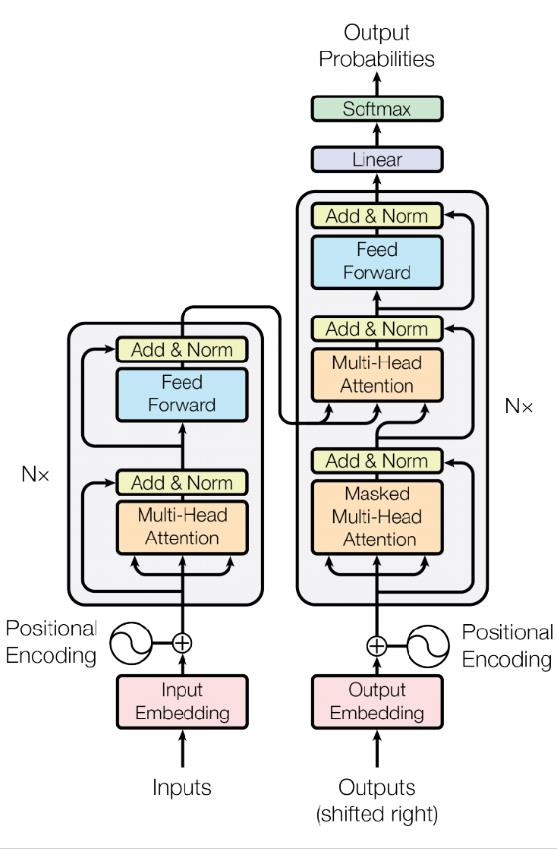
\includegraphics[width=0.4\textwidth]{Fig/Transformer.jpg}
% 	\caption{Transformer model structure}
% \end{wrapfigure}
\subsubsection{Overview of Transformer}
Transformer operates as an Encoder-Decoder model, leveraging an attention mechanism.
In the Encoder-Decoder architecture, the Encoder takes an input sequence and encodes the information into a single context vector. 
Conversely, the Decoder utilizes this context vector to generate an output sequence.
Within the model structure, a crucial component is the "embedding" process. 
This process involves the conversion of input values into a unified vector representation.

The attention mechanism employed by the Transformer is a key feature. 
It assigns varying weights to elements within the input sequence, placing greater emphasis on pertinent information. 
This emphasis is then reflected in the model's output. 
The Transformer employs this mechanism to comprehensively evaluate the significance of the entire input sequence when generating the output.

\subsubsection{Background of employing Transformer}

The decision to employ the Transformer model in stock price prediction stems from its advanced capabilities in handling sequential data. 
While LSTM and GRU have made significant strides in addressing the vanishing gradient problem, they still have limitations, particularly in their sequential processing nature and in fully capturing long-range dependencies.
The expectation is that the Transformer, with its advanced architecture, will outperform traditional models like LSTM and GRU in capturing the intricate patterns and dependencies inherent in stock price data, leading to more accurate and reliable predictions.

\subsection{Loss function}
\begin{figure}
	\centering
	
\includegraphics[width=0.8\textwidth]{Fig/loss_function.png}
	\caption{Huber loss function}
	\label{fig:huber_loss}
\end{figure}

\subsubsection{Overview of Loss function}
In our model, the loss function is defined as:
\begin{equation}
	\mathcal{L} = \mathcal{L}_{H} + \lambda \sqrt{\sum \left( \frac{\hat{y}_{t} - {y}_{t}}{{y}_{t-1} - {y}_{t}} \right)^{2}}
\end{equation}
where $\mathcal{L}_{H}$ is Huber loss function, $\lambda$ is a regularization parameter, $y_{t}$ is the actual value at time step $t$, and $\hat{y}_{t}$ is the predicted value at time step $t$.
The Huber loss function is given by:
\begin{equation}
	\label{eq:huber_loss}
	\mathcal{L}_{H} = \sum_{t=1}^{n} \begin{cases}
		\frac{1}{2}(y_{t} - \hat{y}_{t})^{2} & \text{tf } |y_{t} - \hat{y}_{t}| \leq \delta \\
		\delta |y_{t} - \hat{y}_{t}| - \frac{1}{2}\delta^{2} & \text{otherwise}
	\end{cases}
\end{equation}

The Huber loss function is chosen for its balanced approach, combining the robustness of the L1 norm with the smoothness of the L2 norm. 
This makes it differentiable and less sensitive to outliers in the data. 
Visually, the Huber loss resembles the L2 norm for smaller errors but transitions to an L1 norm-like behavior for larger errors, effectively handling outliers as seen in the Figure \ref{fig:huber_loss}.

Additionally, we incorporated a regularization term into the loss function. 
This term is designed to provide some leniency for rapid changes in stock prices. 
It implies that the model is less penalized for missing rapid price changes, acknowledging the inherent volatility and unpredictability in stock price movements.


\subsubsection{Background of employing Loss function}

Initially, our model employed the Huber loss function without a regularization term. 
However, we observed that the model tended to predict the next day's stock price as being equal to the current day's price, a pattern inconsistent with real-world stock market behavior. 
This phenomenon aligns with the martingale theory in probability, where the expected next value of a sequence of random variables is simply the current value.

Recognizing that stock prices are not merely a sequence of random variables but are influenced by trends and patterns, we introduced the regularization term. 
This addition encourages the model to recognize and respond to short-term trends in stock prices, rather than strictly adhering to the immediate past value. 
It allows the model to be more responsive to rapid changes, aligning its predictions more closely with the dynamic nature of the stock market.


\subsection{VADER}

\subsubsection{Overview of VADER}
VADER (Valence Aware Dictionary and sEntiment Reasoner) is a rule-based model specifically designed for sentiment analysis of social media text. 
It excels in analyzing the sentiment of individual words and phrases, providing an overall sentiment score for the text. 
VADER employs a combination of lexical elements and grammatical heuristics to assess sentiment, effectively capturing both the polarity (positive or negative) and intensity of emotions expressed in the text.

One of VADER's strengths lies in its ability to adeptly handle the unique characteristics of social media text, such as slang, emoticons, and abbreviations, which are often challenging for traditional sentiment analysis models. 
Its performance in sentiment analysis tasks, especially in the context of social media, is notably high. 

\subsubsection{Background of employing VADER}

In our stock price prediction model, we integrated VADER to incorporate additional factors that could influence stock prices. 
While our model effectively captures short-term trends in stock prices—predicting rises or falls based on recent price movements—it sometimes struggles to anticipate when these trends might not hold.

To address this, we turned to external factors like news, which can significantly impact stock prices both in the short and long term. 
News sentiment, whether positive or negative, along with the intensity of the sentiment, can be pivotal in shaping stock market trends. 
VADER's ability to evaluate these sentiments provides a nuanced understanding of how news might affect stock prices.

We use VADER to generate sentiment scores for news articles, incorporating these scores as new factors in our model. 
This approach aims to enhance the model's predictive accuracy by accounting for the influence of news sentiment on stock price movements, capturing new trends that might not be evident from historical price data alone.


\section{Implementation}
\label{sec:Implementation}
\subsection{Data Set}
\subsubsection{Stock Selection}

We selected about 15 stocks from KODEX 200 and S\&P 500 for predicttion. 
Also, we categorized the stocks into two groups: stable stocks and unstable stocks based on the commercial EFT funds holdings.
The following table shows the stocks we selected.


\begin{table}[h]
	\label{tab:example}

	\centering
	\begin{tabular}{cccc}
	\toprule\toprule
	\textbf{Korea} & \textbf{Korea} & \textbf{US Nasdaq} & \textbf{US Nasdaq} \\ 
	\textbf{Stable} & \textbf{unstable} & \textbf{Stable} & \textbf{unstable} \\ 
	\midrule
	Item 1 & Item 2 & Item 3 & Item 4 \\
	Item 1 & Item 2 & Item 3 & Item 4\\
	\bottomrule
	\end{tabular}
\end{table}

\subsubsection{Normalization}



\subsubsection{Training Set}



\subsubsection{Test Set}




\subsection{UI/UX Design}
The user experience (UX) and user interface (UI) aspects of the system were prioritized to ensure a seamless and intuitive user interaction. 
The frontend was designed with a user-centric approach, focusing on usability and visual appeal.
% User research and feedback were considered to create an intuitive navigation flow, clear information hierarchy and visually pleasing design elements. 
The UI elements were designed to be responsive and accessible across different devices and screen sizes, enhancing the overall user experience.

\subsection{Frontend}

\subsection{Backend}
Django, a Python web framework, was employed for server-side development.
% It handles user authentication, routing and business logic implementation. 
% The backend interacts with the database, utilizing SQLite for data storage and retrieval. External APIs are integrated to fetch relevant information for the exchange program and university details. 
% NLP libraries of KoT5 and GPT-4 are utilized for text summarization and analysis. AWS Lightsail provides the infrastructure for hosting the backend server, ensuring reliable and scalable performance. 
% We chose to use AWS server with 1GB RAM, 1 vCPU, and 40GB SSD, as it offers a lightweight and suitable solution for our initial deployment, despite its limitations.

\section{Evaluation}
\label{sec:Evaluation}
\subsection{Evaluation Metric}

\subsubsection{Mean Prediction Accuracy (MPA)}
To assess the effectiveness of our methods, we calculate the Mean Prediction Accuracy (MPA), defined as:
\begin{align}
    \label{eq:MPA}
    \text{MPA}_{t} = 1 - \frac{1}{N} \sum_{i=1}^{N} \frac{|\hat{y}_i - y_i|}{y_i}
\end{align}
where $ N $ is the number of stocks, $ \hat{y}_i $ and $ y_i $ represent the predicted and actual high or low prices, respectively, for the $ t $-th day of stock $ i $.

\subsubsection{Mean Absolute Error (MAE)}
The Mean Absolute Error (MAE) is another metric used to evaluate our methods:
\begin{align}
    \label{eq:MAE}
    \text{MAE}_{t} = \frac{1}{N} \sum_{i=1}^{N} |\hat{y}_i - y_i|
\end{align}
Here, $ N $ denotes the number of stocks, with $ \hat{y}_i $ and $ y_i $ being the predicted and actual high or low prices for the $ t $-th day.

\subsubsection{Trend Accuracy (TAC)}
Given our focus on short-term stock price trends, we also compute the Trend Accuracy (TAC):
\begin{align}
    \label{eq:TAC}
    \text{TA}_{t} = \frac{1}{N} \sum_{i=1}^{N} \mathbb{1}(\text{sign}(\hat{y}_i - \hat{y}_{t-1}) = \text{sign}(y_i - y_{t-1}))
\end{align}
where $ N $ is the number of stocks, $ \hat{y}_i $ and $ y_i $ are the predicted and actual high or low prices for the $ t $-th day, and $ \mathbb{1}(\cdot) $ is the indicator function.

\subsubsection{Accuracy}
To compare the similarity between the predicted and actual price intervals, we calculate the accuracy(ACC):
\begin{align}
    \label{eq:accuracy}
    \text{Accuracy}_{t} = \frac{1}{N} \sum_{i=1}^{N} \frac{\text{length}(\{ y_{\min}<y<y_{\max} \cap \hat{y}_{\min}<y<\hat{y}_{\max} \})}{\max(\text{length}(\hat{y}_{\min}<y<\hat{y}_{\max}), \text{length}(y_{\min}<y<y_{\max}))}
\end{align}
where $ N $ is the number of stocks, $ \hat{y}_{\min} $ and $ \hat{y}_{\max} $ are the predicted minimum and maximum prices for the $ t $-th day, and $ y_{\min} $ and $ y_{\max} $ are the actual minimum and maximum prices for the $ t $-th day.

\subsection{Result}


\begin{table}[h]
	\label{tab:result}
	\centering
	\begin{tabular}{c|c|c|c|c|c|c|c|c|c}
	\toprule\toprule
	% \multirow{2}{*}{\textbf{Model}}
	\multicolumn{2}{c}{}& \multicolumn{4}{|c|}{\textbf{STABLE}} & \multicolumn{4}{c}{\textbf{UNSTABLE}} \\
	\midrule
	\multicolumn{2}{c|}{\textbf{Model}} & \textbf{MPA} & \textbf{MAE} & \textbf{TAC} & \textbf{ACC} & \textbf{MPA} & \textbf{MAE} & \textbf{TAC} & \textbf{ACC} \\ 
	\midrule
	\multirow{ 2}{*}{\textbf{LSTM}} & High			& 	0.9922& 	1.2179& 	0.5640& \multirow{ 2}{*}{0.4183}
					  								& 	0.9856& 	4.2027& 	0.5872& \multirow{ 2}{*}{0.4163}	\\ 
									& Low			& 	0.9921& 	1.1985& 	0.5702& 
					  								& 	0.9851& 	4.1493& 	0.5711& 							\\ 
	\multirow{ 2}{*}{\textbf{GRU}} 	& High			& 	0.9929& 	1.1118& 	0.5640& \multirow{ 2}{*}{0.4340}	
													& 	0.9864& 	3.9909& 	0.5930& \multirow{ 2}{*}{0.4199} 	\\ 
									& Low			& 	0.9926& 	1.1193& 	0.5659& 	
													& 	0.9862& 	3.8426& 	0.5747& 							\\ 
	\multirow{ 2}{*}{\textbf{Transformer}} 	& High	& 	0.9906& 	1.4721& 	0.4743& \multirow{ 2}{*}{0.4295}	
													& 	0.9827& 	5.2046& 	0.4731& \multirow{ 2}{*}{0.3374} 	\\ 
											& Low	& 	0.9892& 	1.6502& 	0.5361& 
													& 	0.9830& 	4.8531& 	0.4616& 							\\ 
	\midrule
	\multicolumn{ 2}{c|}{\textbf{BASELINE}}			& 	0.9815& 		 & 		 & 	
					  								& 	0.9815& 		 & 		 & 									\\
	\bottomrule
	\bottomrule
	\end{tabular}
	% \caption{Result of our models}
\end{table}
As shown in Table \ref{tab:result}, the performance of our models on the test set is quantified. Incorporating VADER into the model has resulted in MPA surpassing that of the baseline model, which is DP-LSTM. 
Notably, the model's performance varies based on the stability of the stocks. For unstable stocks, the MAE significantly increases, and ACC decreases.
Both LSTM and GRU models exhibit similar performance metrics, whereas the Transformer model demonstrates slightly lower performance compared to the other two models. 


\section{Limitation and Discussions}
\label{sec:Limitation}
\subsection{Prediction Quality}

\begin{figure}
	\centering
	
\includegraphics[width=0.8\textwidth]{Fig/unstable_AAPL.png}
	\caption{}{}
	\label{fig:AAPL}
\end{figure}

As illustrated in Figure \ref{fig:AAPL}, our models demonstrate a tendency to follow the trend of stock prices. 
If the stock price has been increasing up to the current day, the model predicts a continued increase for the next day, and similarly for a decreasing trend. 
This indicates that the models are effectively capturing the short-term trend of stock prices rather than merely reflecting random fluctuations. 
However, it's noteworthy that while the models occasionally attempt to predict price rebounds, these predictions are not consistently successful.

The impact of incorporating VADER for sentiment analysis on stock price prediction is not definitively clear. 
Although the sentiment score is more aligned with long-term trends, the models still achieve a higher MPA score compared to the BASELINE model. 
This suggests a potential, albeit indirect, benefit of including sentiment analysis in the prediction process.

A challenge arises when the stock price remains relatively constant with minor fluctuations. 
In such scenarios, the models often predict in the opposite direction of the actual trend, leading to inaccuracies. 
This issue is particularly evident in the period from November 16, 2023, to December 1, 2023, as shown in Figure \ref{fig:AAPL}.

Regarding the comparison of LSTM, GRU, and Transformer models, LSTM and GRU exhibit similar prediction quality, but the Transformer model lags slightly behind. 
As indicated in Table \ref{tab:result}, the Transformer model has a higher MAE and lower scores in MPA, TAC, and ACC compared to LSTM and GRU. 
Notably, the Transformer model's predicted price range (high to low) is broader and less consistent than the other models, leading to more frequent misses in trend prediction. This results in its lower TAC and ACC scores.

Despite these challenges, the Transformer model holds promise, particularly due to its capability to interpret long-term trends and its flexibility in integrating additional features. 
In our project, we limited the input features to stock prices and sentiment scores, which may not fully leverage the Transformer model's potential. 
Future improvements and the inclusion of more diverse features could enhance the Transformer model's applicability in real-world scenarios.

\subsection{Lack of Information}

A significant challenge in our project arises from the constraints in collecting sentiment scores using the VADER model. 
For this purpose, we sourced news articles from the Investing.com website (\url{investing.com}). However, we encountered a limitation in the availability and distribution of these articles. 
The website provides approximately 1000 news articles per stock, but this distribution is highly uneven across different stocks. For instance, stocks like AAPL and TSLA have a daily influx of articles, whereas other stocks receive considerably less coverage. 
This disparity in news frequency is a primary reason why we could not effectively apply the VADER model to stocks in the KODEX 200, limiting our analysis and results.

Another constraint is the temporal availability of news articles. The website only offers access to current day's news, preventing us from utilizing historical data in our training set. 
The ability to access past news articles would significantly enhance our model's training process, allowing us to incorporate sentiment scores from earlier periods. 
This would likely improve the model's ability to understand and predict stock price movements based on a more comprehensive historical context.
Furthermore, access to professional analysts' reports could potentially elevate the prediction quality of our model. 


\section{Related Work}
\label{sec:Related_Work}
% \subsection{Stock Price Prediction}
% Stock Price Prediction is the task of forecasting future stock prices based on historical data and various market indicators. 
% It involves the use of statistical models and machine learning algorithms to analyze financial data and make predictions about a stock's future performance. 
% Stock price trends are influenced by numerous factors, including interest rates, inflation rates, and financial news. 
% To make accurate stock price predictions, one must leverage this diverse set of information. 
% In the banking industry and financial services sector, teams of analysts are dedicated to scrutinizing, analyzing, and quantifying qualitative data from news sources. 
% A substantial amount of information regarding stock trends is extracted from the extensive corpus of textual and quantitative data involved in such analysis.

Recent research trends in stock price prediction include advancements in deep learning-based regression models. \cite{li2019dp}
These models often utilize Long Short-Term Memory (LSTM) networks and innovative validation techniques, such as walk-forward validation, to enhance their predictive capabilities.

In addition, some researchers have explored Particle Filter Recurrent Neural Networks (PF-RNNs), a new RNN family explicitly designed to model uncertainty within their internal structure. \cite{ma2020particle}
Unlike traditional RNNs that rely on a deterministic latent state vector, PF-RNNs maintain a latent state distribution approximated as a set of particles. 
To enable effective learning, researchers have introduced a fully differentiable particle filter algorithm that updates the PF-RNN latent state distribution based on Bayes' rule. 
Experimental results have shown that PF-RNNs can outperform conventional gated RNNs across various domains, 
including synthetic robot localization datasets and real-world sequence prediction tasks, which is stock price prediction.

Furthermore, recent studies have proposed novel approaches, such as the development of a sentiment-ARMA model, which combines the autoregressive moving average model (ARMA) with sentiment analysis of financial news articles. \cite{mehtab2021stock}
This model is integrated into an LSTM-based deep neural network consisting of three components: LSTM, VADER model, and a differential privacy (DP) mechanism. 
The proposed DP-LSTM scheme has demonstrated the potential to reduce prediction errors and enhance model robustness. Extensive experiments conducted on S\&P 500 stocks have indicated promising results, 
including a 0.32\% improvement in mean Mean Percentage Absolute Error (MPA) 
and a significant up to 65.79\% reduction in Mean Squared Error (MSE) for the prediction of the market index S\&P 500.



\section{Conclusion}
\label{sec:Conclusion}
In conclusion, our project has focused on predicting the short-term movements of blue-chip stocks, a strategy that has proven effective over periods ranging from a few days to a few months. 
To achieve this, we have leveraged advanced machine learning techniques, employing models: LSTM, GRU, and Transformer.

Additionally, we integrated VADER, a sentiment analysis tool, to incorporate the impact of recent events and news on stock prices. 
This integration aimed to capture both short- and long-term changes in stock prices influenced by current events. 
While our results have been promising, there is potential for further improvement. 
Enhancing the feature set, particularly for the Transformer model, could yield more accurate predictions. 
Access to historical news articles and professional analysts' reports would also significantly enrich our dataset, potentially leading to more nuanced and informed predictions.

Our prediction results are available on our website, \url{http://3.34.75.210:8000/}.

\bibliography{reference}

\end{document}
